\documentclass[twoside]{article}
\usepackage{float}
\usepackage{graphicx}
\usepackage{framed}
\usepackage[a4paper, total={6.4in, 8in}]{geometry}


\usepackage{amsmath}
\usepackage{subfig}
\usepackage{multicol}
\usepackage{fancyhdr}
\usepackage[utf8]{inputenc}
\pagestyle{fancy}

\fancypagestyle{firststyle}
{
	\fancyhead{}
	\fancyhead[L]{Sabancı University Program for Undergraduate Research (PURE)}
		\fancyhead[R]{Fall 2017-2018}
}
\fancyhead{}
\fancyhead[CE]{Yıldırır,Taşyaran}
\fancyhead[CO]{Analysis of Data Sketches}

\setlength{\oddsidemargin}{\evensidemargin}  

\renewcommand{\headrulewidth}{1pt}
\renewcommand{\footrulewidth}{0pt}
%\usepackage{biblatex}
%\addbibresource{References.bib}
\bibliography{bibliography}
\usepackage[
style=apa,
backend=biber,
sortcites=true,
sorting=nyt,
%    isbn=false,
%    url=false,
%    doi=false,
%    eprint=false,
hyperref=false,
backref=false,
%    firstinits=false,
]{biblatex}

\begin{document}
	\thispagestyle{firststyle}
	\begin{figure}
	

\textbf{Fatih Taşyaran} \hfill fatihtasyaran@sabanciuniv.edu \\
\hfill	\textit{Computer Science and Engineering,2014} \\
\textbf{Kerem Yıldırır} \hfill keremyildirir@sabanciuniv.edu \\
\hfill	\textit{Computer Science and Engineering,2015} \\
\textbf{Kamer Kaya} \par
\textit{Computer Science and Engineering}
	
	\end{figure}
	\section{Abstract}
	One of the biggest challenges in today's business and technology world is dealing with enormous chunks of data. One of the problems people encounter while working with big data is that it takes too much time to analyze it. Standard data structures like linked lists and hash tables may be incompetent or inefficient for some specific problems such as keeping track of the elements' frequency, or checking if an element is in the set or not. Hence, people are trying  to come up with clever solutions such as data sketches. We implemented various sketches, and analyzed their performance for possible improvements.
\section{Introduction}

Data sketches are derived from Bloom Filters, which are arrays that consist of 1 and 0s (Cormode, 2017). Bloom Filters are used in search and validation purposes. Bloom Filters(BF) can answer a query with 2 possible outputs: \begin{itemize}
	\item The element is definitely not in the data
	\item The element is probably in the data 
	
\end{itemize}
 In ideal case, for $i$th element in the data, $BF[i]=1$. On the contrary, in real data, this is rarely the case. Even on hash table applications, there exists an item $i$ such that $h_{i}=h_{j}$. Still,
 BM's are compact, nice structures. (Cormode, 2017)


Sketches are data structures which are used for following the frequencies of elements in a large data set. Main distinguishing feature of a sketch is that its size does not depend on size of the data set. Size of the sketch depends on two error parameters: $\delta$ and $\epsilon$, where $\epsilon$ is the minimum error rate  user can afford
and $\delta$ is the error frequency. 
Number of rows and columns in the sketch is computed with the following formulas: $$nrows=\log_{2}(\frac{1}{\delta})$$ 
$$ncols=\frac{2}{\epsilon}$$
A step by step explanation for sketch mechanism is  as follows:
\begin{itemize}
\item Define sketch size with $\delta$ and $\epsilon$
\item Insert elements into the sketch table using predefined number of hash functions and perform the operation on table in order to keep the frequency. (Different sketches use different operations.(Cormode, 2017))

\end{itemize}
There are various hash functions for this purpose, but in this paper, our choice was Tabular Hashing. The reason behind this choice  is ,Tabular Hashing is simple, robust and easily implemented. We managed to improve total performance by merging the hash functions' tables, which led to a significant improvement performance-wise.
\section{Implemented Data Sketches}
\subsection{Count-Min Sketch}
In the application of this sketch, the element to be inserted is hashed $n$ times, where $n$ represents the number of rows. Each element is hashed by hash functions $h_{1},h_{2} \dots h_{n}$. Each hash function increments  $sketch[i][h_{i}]$ where $i$ corresponds to  hash function's return value and $sketch$ refers to the sketch table. For queries, the minimum corresponding value of all rows is returned.(Cormode, 2017)
\begin{figure}[H]
	\centering
	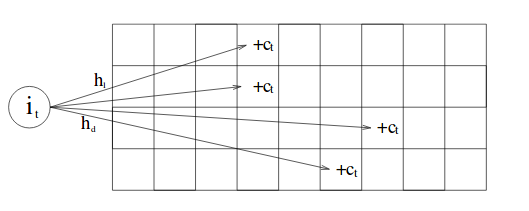
\includegraphics[width=0.5\textwidth]{Countmin.png}
	\caption{Illustration of Count-Min Sketch}
	

\end{figure}
\subsection{Count-Mean Min Sketch}
Initialization of Count-Mean Min Sketch(CMM) is exactly same as Count-Min Sketch(CM). It can be said that since every index is incremented for multiple elements, CM's results are \textit{overestimating} the true values. Hence it is a biased estimator. CMM intends to solve this problem by subtracting a noise from the queried value. Noise is estimated as : $\frac{NoElements - sketch[i][h_{i}]}{ncols- 1}  $ for every row. After calculating the noise, it is deducted from each $sketch[i][h_{i}]$ value computed in each row. Finally, the minimum of these values is returned as query output.$$
output=\min(sketch[i][h_{i}]-noise_{i})\quad i=1 \dots nrows$$ where $i$ is the row number and $h_ {i}$ is the index obtained from hash function. (Deng,Rafiei, n.d)


\subsection{Count Sketch}
In Count Sketch, 2 hash functions are maintained for each row. $h_{k}$ for determining the column index value, and $g_{k}$ for determining an increment value in the interval $[-1,1]$.is done by acquiring the median of all $sketch[i][h_{i}]$.
$$sketch[k][h_{k}]=sketch[k][h_{k}]+ g_{k} \quad  k=1 \dots nrow$$
It aims to neutralize the bias that comes with overestimating. (Cormode,Hadjieleftheriou, 2008)
\subsection{Count-Min Sketch with Conservative Update }
This is an update for Count-Min Sketch and aims to solve the unnecessary incrementation in the sketch. Since queries return the minimum of $sketch[i][h_{i}]$, during the incrementation, it only increments the minimum value of all $sketch[i][h_{i}]$. In other words, only $\min (sketch[i][h_{i}])$ is incremented. This heuristic reduces the bias caused by overestimating.(Goyal, 2012)
\section{Tabular Hashing}
In data sketches, elements that inserted to the  table must be hashed multiple times. In this implementation of sketching, tabular hashing is used. Which first introduced in an article by Zobrist to avoid recalculations of board configurations at the current state in board games.(Thorup, 2012) It is a  strong hash function which grants significant level of randomness. Hashing  process requires a table filled with random integers.  After  initializing the table, hash function can be used. Code for hashing can be
examined in the following figure.
\begin{figure}[H]
	\centering
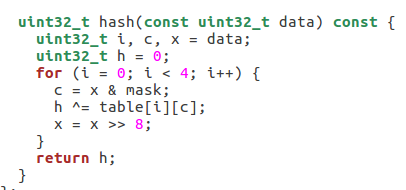
\includegraphics[width=0.5\textwidth]{hashhh.png}
\caption{Hash function written in C++}
\label{fig:hash}
\end{figure}

With using the fastest known hashing scheme multiplication-shift hashing. Hash function takes an 32-bit integer $x$ as input. It divides $x$ into 4 8-bit chunks and iterates them in order. At each iteration, logical AND operation is done between the element and an 8-bit mask which consists of zeros.
With this, it is guaranteed that first 8-bits of the 32-bit integer becomes zero. This also changes the value of element $x$, to another integer $c$. Then, logical XOR operation is applied between changed element and the integer in hash table which is on the $ith$ row where $0<i<4$ and $cth$ column and assigned to a variable $h$. At the end of iteration, $x$ is shifted right 8-bits. When all iterations are done a unique $h$ value has been achieved.



\section{Parallelization}
The sketch can be seen as a sum of arbitrary sketches using the same $h_{j}$ for their rows $j$. In this manner every sketch is combinable while they use same $\epsilon$, $\delta$ and hash function $h_{j}$ for their rows $j$.
Say in sketch $A$, $A[j,k]$ is the sum of updates to the location $(j,k)$ for index values $i$ such that $H_{j}(i) = k$ in the process and $a_{j,k}$ is a binary vector such that $a_{j,k} = 1$ if and only if $h_j(i) = k$.
Then we can say $$A[j,k] = \sum_{{i=0}}^{{n}}a_{n}[j,k]$$
(Cormode, 2017)
This led us an important consequence that sketches have high potential of parallelization. Since the data is shared between threads that all have their own sketch then combined in order to form a final table by OpenMP's fork-joint parallelism, we can distribute the input set to the threads, as many as available.
\par The drawback here is, while the threads are increasing and subsets of the input set that computed parallel are increasing, memory required to contain their tables are also increasing. This called time-memory trading. In our project, we focus on multi-table computing of sketches, we use more memory but get improvements on performance.

\subsection{Synchronization Problems With Parallelization}
\subsubsection{Race Condition}
In multi-thread programs, threads are communicate by sharing variables. In cache, threads are interleaving. Basically saying, there is no defined schedule for which thread is processing at the time or in which sequence they will be processed. Thus when the scheduling of threads affect the output, this ambiguity may result in different outputs of the same program at different runs. This is called a race condition.
\subsubsection{False Sharing}
In symmetric multiprocessor systems, each processor has a local cache. And the memory system must guarantee a consistency between the data in this caches, called cache coherency protocol. When threads on different processors modify variables that sits on the same cache line, a false sharing occurs. This invalidates the cache line and forces an update on cache line. Thus the false sharing causes cache lines to go back and forth between threads and decreases performance.
\subsubsection{Synchronization Tools}
\textbf{Synchronization} is bringing one or more threads to a well defined and known point in their execution. Common synchronization tools are:
\begin{itemize}
	\item \textbf{Barrier:} Each thread wait at the barrier until all threads arrive.
	\item \textbf{Mutual Exclusion:} Defining a block of code that only one thread at a time can execute.
	\item \textbf{Critical:} Defines a mutual exclusion for a block of code.
	\item \textbf{Atomic:} Uses hardware support to do a quick update on a value. If there is no hardware support, act like critical. Only use a scalar l-value and a non overloaded built-in operator.
	\item \textbf{Lock:} Lowest level mutual exclusion in synchronization. Lock is actually a variable. The thread that holds the lock can execute processes on the lock and the other threads doing something else while waiting for lock is available. 
	
\end{itemize}

\section{Parallelization With Synchronized Hashing}
As mentioned before, we focus on multi-table sketches in our project and gain performance while using more memory. Moreover we develop a new way of tabular hashing in order to exploit the speed of fastest L1 Cache. In our model of tabular hash, instead of using different randomly-filled tables for each row of the sketch as a look-up table for corresponding row's hash function; we merged these tables by arrange the columns of tables of rows consecutively.
\begin{figure}[H]
	\centering
	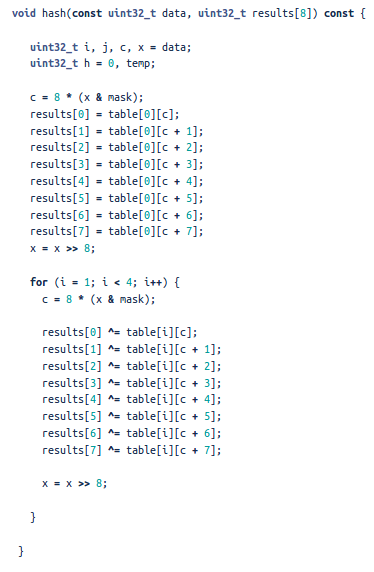
\includegraphics[width=0.4\textwidth]{mergedhasher.png}
	\caption{Code for merged tabular hashing}
	
	\label{fig:code}
\end{figure}

\begin{figure}[H]
	\centering
	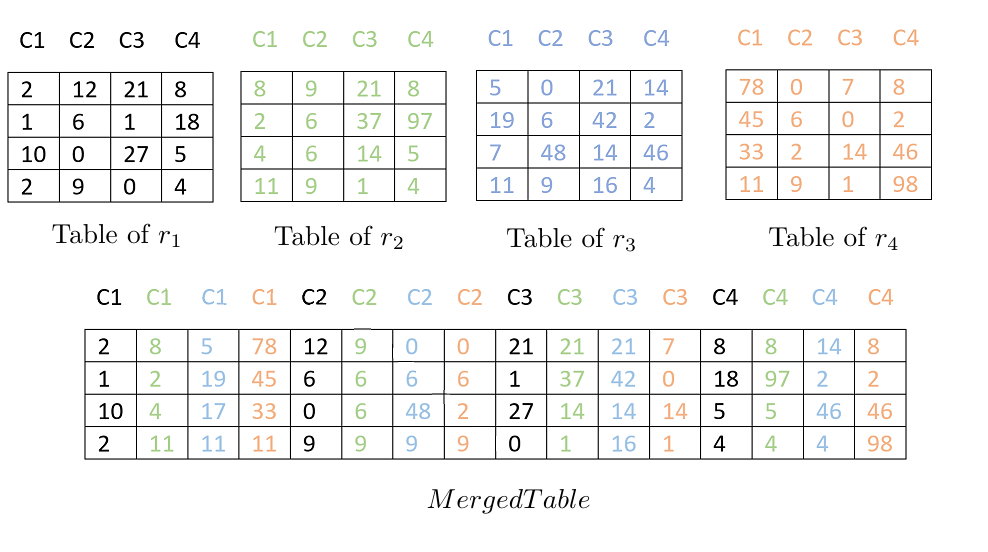
\includegraphics[width=0.8\textwidth]{illustration.png}
	\caption{Illustration of Merging Tables of Rows}
	
	
\end{figure}

\par 
In the figure \ref{fig:code}, implementation of merged hasher can be seen. Since row size has been fixed to 8, results of hash functions are put side by side in the hash table.
The advantage of our method is, instead of different threads to read data that sits on different cache lines, all threads read data from the same cache line. That will be on the fastest L1 cache during process. Expecting result is reducing in cache-misses thus increase in performance.
This result could be seen in experiments section.


\section{Experiments}

We ran our experiments, on the Gandalf computer in Sabanci University which has the following specs:

\begin{framed}
	\textbf{System:} CentOS \texttt{x86\_64}, \texttt{Linux 2.6.32-431.e16.x86\_64} \par
	\textbf{CPU:} Intel(R) Xeon(R) CPU E7-4870 v2 @ 2.30 GHz x2 \par
				  30 Cores, 60 Threads \par
	\textbf{Compiling:} GCC 5.3.0, C++11, OpenMP \par
	\textbf{Memtotal:} 529170124 kb \par
\end{framed}

To calculate the speed-up we used the following formula:

\par $$T_{s} =\text{Non-parallel execution time}$$
$$T_{n} = \text{Execution time using $n$ threads} $$
$$SpeedUp = \frac{T_{s}}{T_{n}}$$

We also fixed our sketches size to 8 by 211 in order to facilitate coding and track results more precisely while developing the new method.

\subsection{Results}

\begin{figure}[H]
	\centering
	\subfloat{{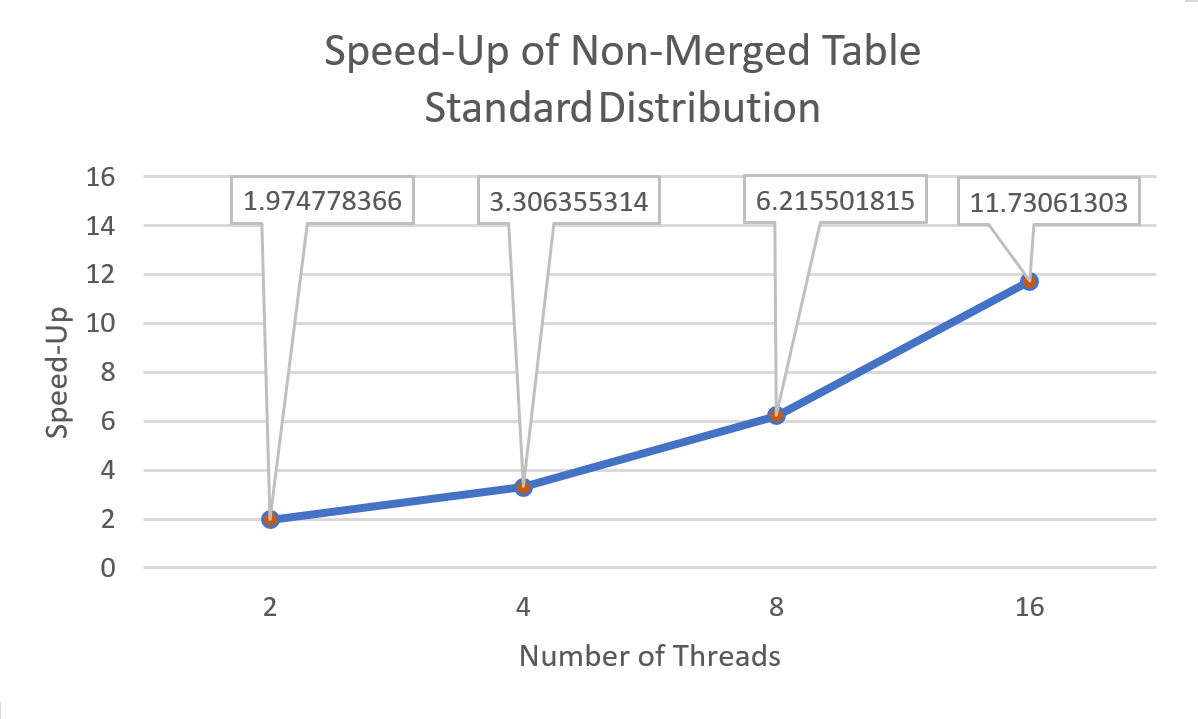
\includegraphics[width=7cm]{sup-chart-nonmerged-standart} }}%
	\subfloat{{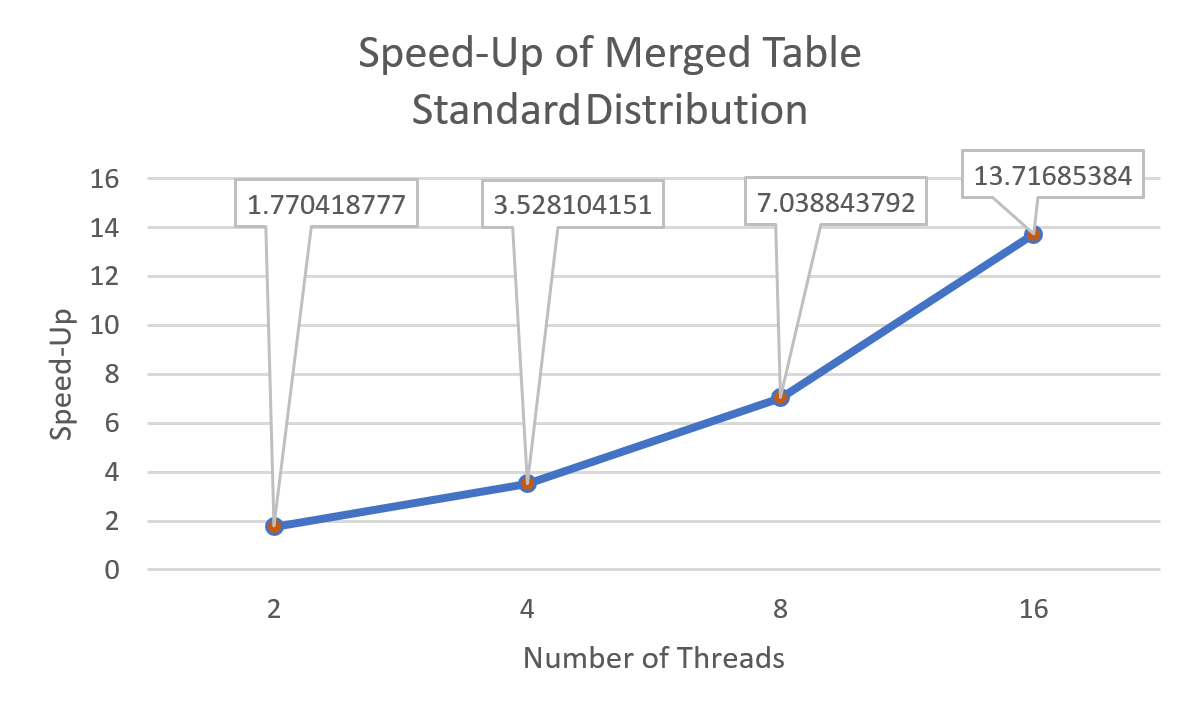
\includegraphics[width=7cm]{sup-chart-merged-standart} }}%
	\caption{Experiment Results Averaged For 10 Repetition}
\end{figure}

\par As could be seen in the results, our offered method becomes faster as number of threads are increasing. This is due to more efficient usage of L1 Cache as mentioned before.

\par The performance increase is even clearer in uniform distribution. In standard distribution, due to high repetition of input values, cache lines that contains parts of tables that associated with hashing of repeated values rows are tend to stay in L1 cache. But as uniformity increases, more different cache lines are invoked by different threads and this cause cache lines to go back and forth in the cache -not same as false sharing-. This result also shows that our model's sit on the L1 cache aim is successful.

\begin{figure}[H]
	\centering
	\subfloat{{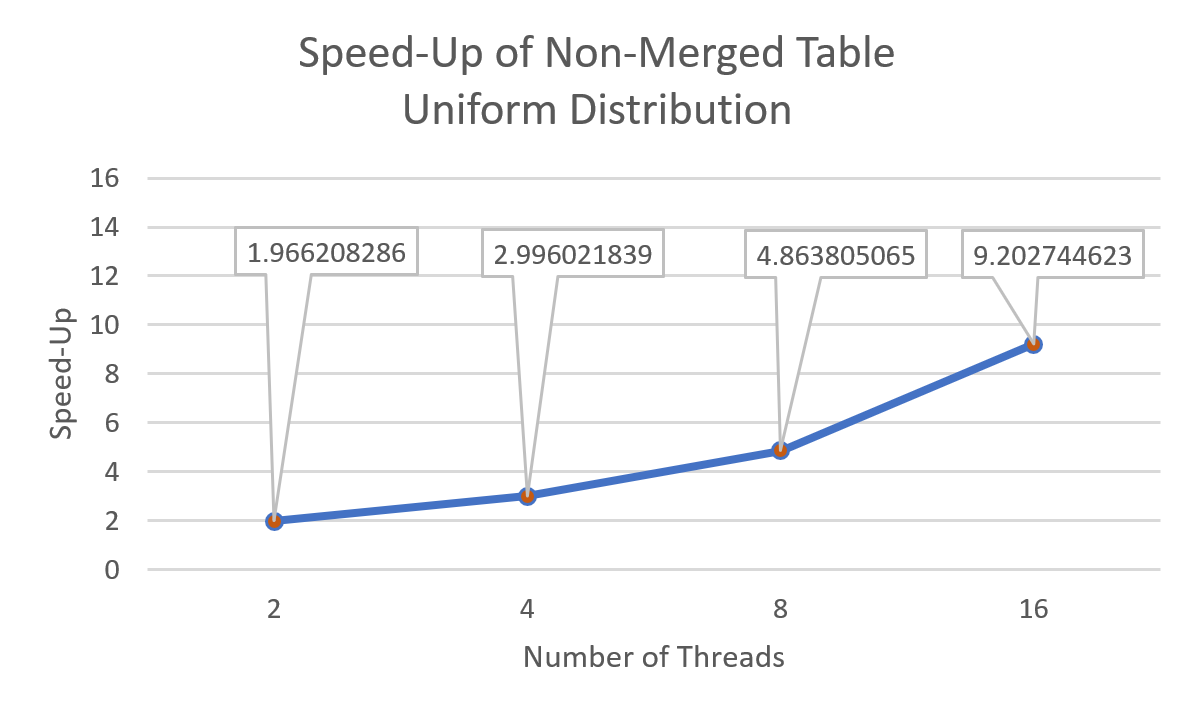
\includegraphics[width=7cm]{sup-chart-nonmerged-uniform}}}%
	\subfloat{{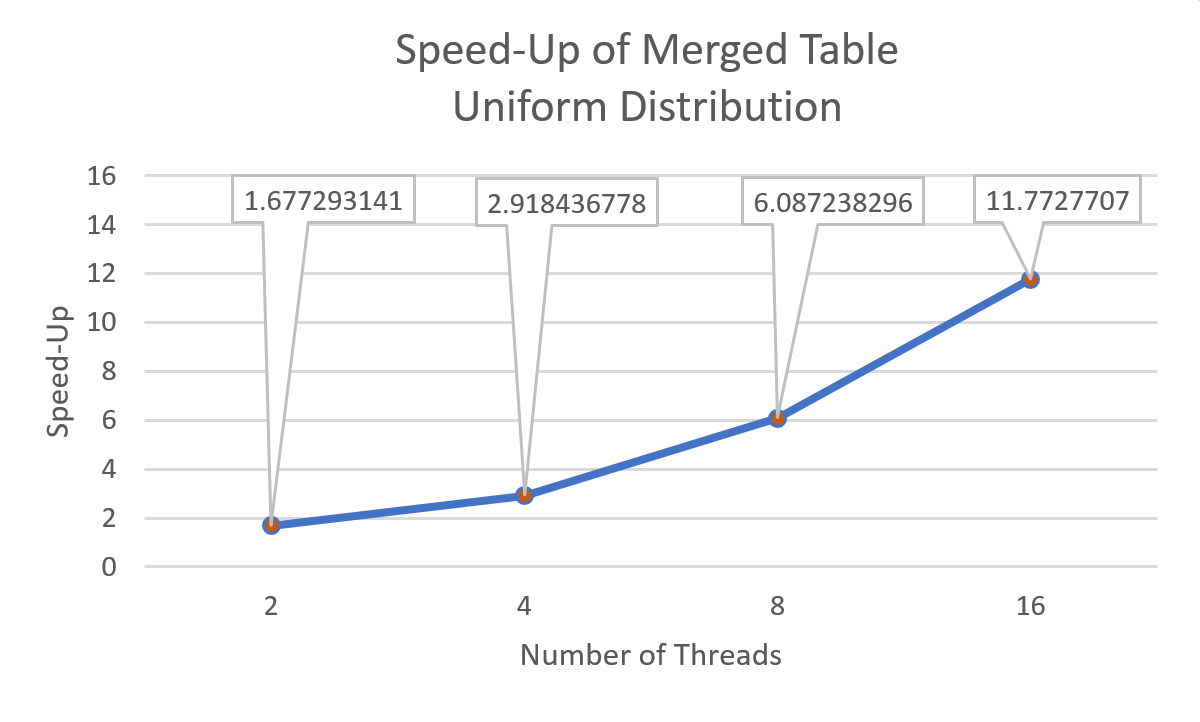
\includegraphics[width=7cm]{sup-chart-merged-uniform} }}%
	\caption{Experiment Results Averaged For 10 Repetition}
\end{figure}


\par Errors are also exactly same pairs for two set of experiments. Since they use practically same tables for hash functions.

\begin{figure}[H]
	\centering
	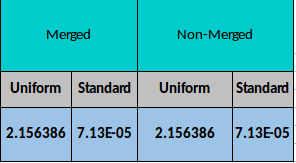
\includegraphics[width=0.6\textwidth]{errors.png}
	\caption{Errors Averaged For 10 Repetitions For Each Set of Experiment}
\end{figure}

\par Higher error rate in experiments using uniform distribution is because count-min sketch is a data type that is more precise in detect heavy-hitters.


\begin{figure}[H]
	\begin{multicols}{2}


\subfloat{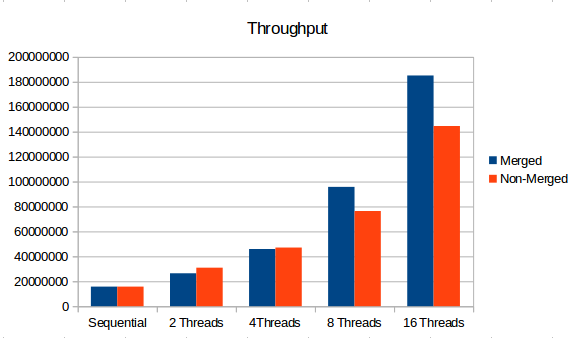
\includegraphics[width=6cm]{histogram.png}}
		
\subfloat{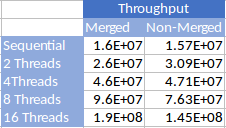
\includegraphics[width=5.5cm]{table.png}}



\end{multicols}
\caption{Throughput comparison for 10 Repetitions For Each Set of Experiment}
\end{figure}

In all experiments we used $2^{30}$ stream size and $2^{25}$ universal set size.

\section{Conclusion and Future Improvement}
To sum up, we experimented with various data sketches and analyzed their performance. On top of that, we came up with a merging method for hashing which is based on the assumption that it will increase the performance, and confirmed it. For future improvement, our aim is to increase the performance even more, and run these applications on card sized mini computers such as Raspberry Pi and Odroid. For the purpose of reproducible researching, source code of the project will be posted on BitBucket and GitHub	.

\section{References}
\begin{itemize}
\item Goyal, A., Daume, H.,  Cormode, G. (2012, July). Sketch Algorithms for Estimating Point Queries in NLP. Retrieved from http://www.umiacs.umd.edu/~amit/Papers/goyalPointQueryEMNLP12.pdf
\item Pǎtraşcu, M.,  Thorup, M. (2012). The Power of Simple Tabulation Hashing. Journal of the ACM, 59(3), 1-50. doi:10.1145/2220357.2220361
\item Thorup, M. (2017). Fast and powerful hashing using tabulation. Communications of the ACM, 60(7), 94-101. doi:10.1145/3068772

\item Cormode, G. (2017). Data sketching. Communications of the ACM, 60(9), 48-55. doi:10.1145/3080008 

\item 
Cormode, G., \& Hadjieleftheriou, M. (2008, August). Finding Frequent Items in Data Streams. AT\&T Labs–Research. Retrieved from http://www.vldb.org/pvldb/1/1454225.pdf
\item

Deng, F., \& Rafiei, D. (n.d.). New Estimation Algorithms for Str eaming Data: Count-min Can Do More. Retrieved from http://citeseerx.ist.psu.edu/viewdoc/download?doi=10.1.1.420.449\&rep=rep1\&type=pdf


\end{itemize}

\end{document}